{\fontsize{12pt}{22pt} \textbf{Principal component Analysis}\par}

\vspace{5mm}

The PCA's objective is to get an approximation of a set of points in a \textbf{low} dimensional set. \\

\underline{Inertia} \\

Inertia $I_g = \Sigma_{i=1}^n p_i ||x_i - g||_M^2$ \\

where $g^T = (\bar{x}^{(1)},...,\bar{x}^{(p)})$ also called the \textit{gravity center}. \\

--> The inertia is thus the weighted average of the squared distance of each observation with the gravity center. \\

--> $p_i$ is the weight given to each observation. Most of the times, $p_i = \frac{1}{n}$ (every observation contributes equally to the analysis) \\

-->  the distance $||.||$ depends on the choosen metric $M$ \\

\underline{Projection} \\

In order to represent the set of points in a low dimensional set, we use projections. \\

The projection should distort the initial set the less as possible, that is:

=> reduce the projection distances as much as possible

=> maximize the average of squared distances between projected points

=> maximize inertia of the projected points \\

In the below figure, maximizing the inertia leads to choosing the projection on the right since d2 > d1.

\begin{center}
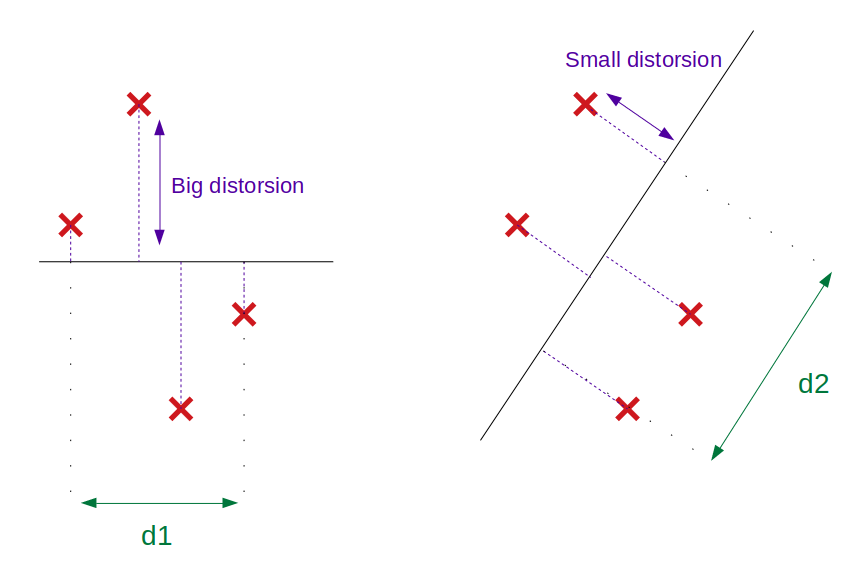
\includegraphics[scale=0.4]{PCA_projections.png}
\end{center}

\underline{Optimisation} \\

If the data are centered, we can also write $I_g = \Sigma_{i=1}^n p_i x_i^T M x_i$ \\

Exprimer l'inertie en fonction de la matrice de covariance.

Exprimer la matrice de covariance du nuage de points projetés.

Exprimer l'inertie en fonction de la matrice de covariance projetés.

Maximiser l'inertie...

\vspace{5mm}